\subsection{Conditioned cross-version comparison}
Across the tested 100-Mbps matrix, equal-RTT total goodput remains close to
the bottleneck for all four implementations, while flow shares and Jain
fairness vary with RTT asymmetry, queue setting, and implementation. Under
the 40- and 80-ms second-flow conditions, the observed long-RTT share differs across implementations. E1 quantifies allocation under RTT asymmetry; E2 evaluates coexistence
with CUBIC at equal RTTs in the documented implementation environments.

For the no-ECN BBR/CUBIC comparison, total goodput is similar across the
four implementation environments, while the BBR/CUBIC share and Jain
index remain condition dependent. The experimental supplement contains the per-run rates, condition
summaries and plotting scripts.

\begin{figure}[htbp]
\centering
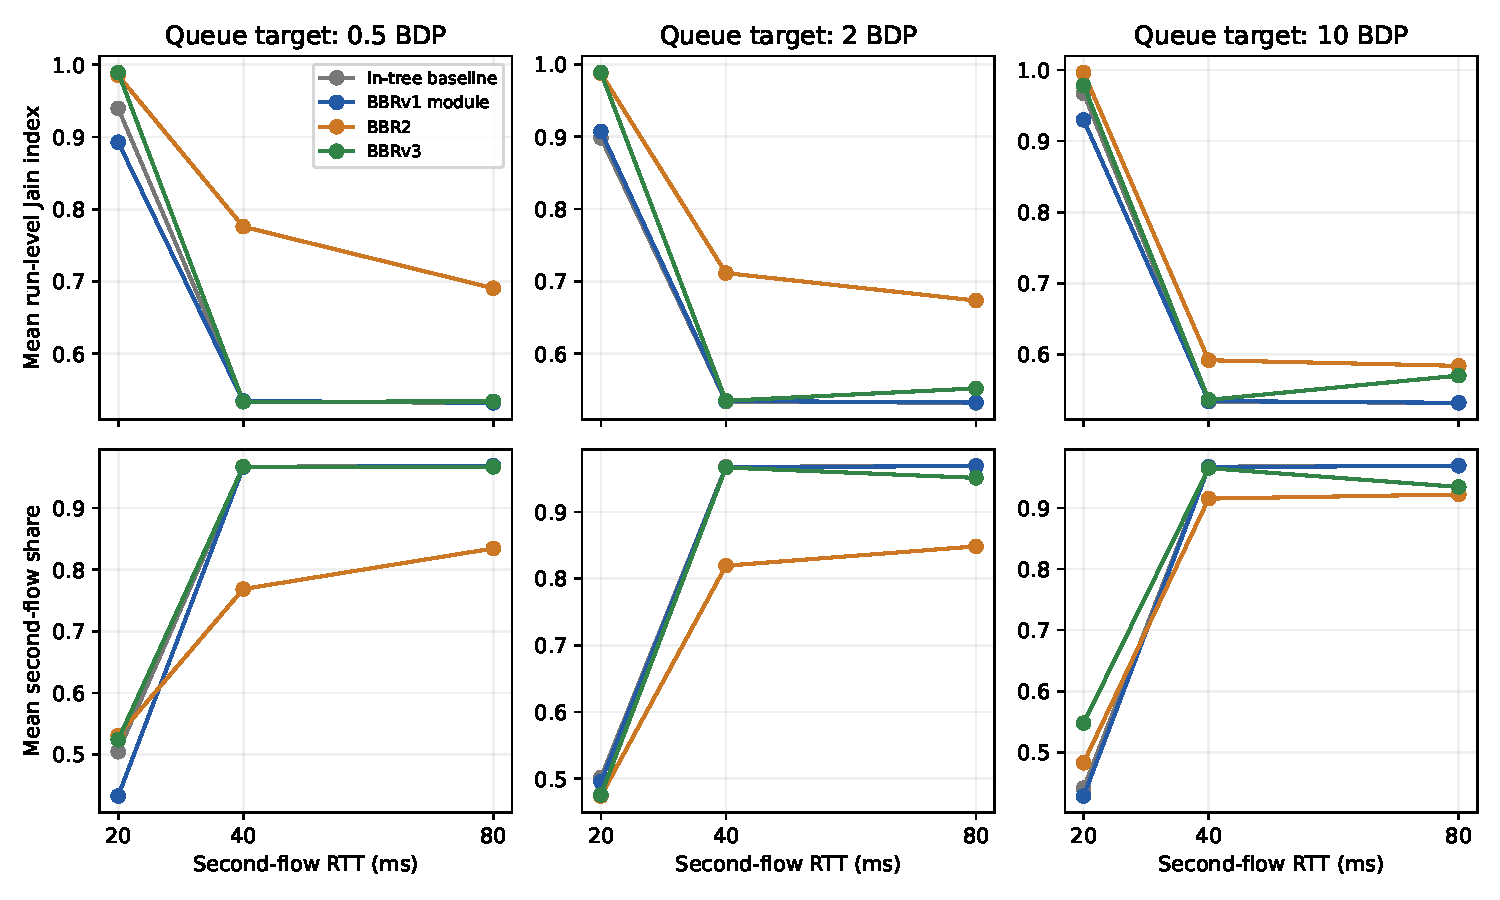
\includegraphics[width=\linewidth]{e1_results.pdf}
\caption{E1 two-flow comparison at 100 Mbps, with first-flow RTT 20 ms and ECN disabled. Curves show means of five run-level Jain indices and second-flow shares, not indices computed from averaged rates. Queue targets use the reference BDP.}
\label{fig:e1_results}
\end{figure}

\begin{table}[htbp]
\centering
\caption{E2 competition with CUBIC at 100 Mbps and equal 20-ms RTTs, with ECN disabled. Each cell summarizes five full-run receiver measurements. Share denotes the BBR flow; Jain is the mean of per-run indices. Different implementation environments limit causal version attribution.}
\label{tab:e2_results}
\small
\begin{tabular}{lrrrr}
\toprule
Implementation & Q/BDP & Total (Mbps) & BBR share & Jain \\
\midrule
In-tree baseline & 0.5 & 95.59 & 0.155 & 0.677 \\
In-tree baseline & 2 & 95.59 & 0.153 & 0.674 \\
In-tree baseline & 10 & 95.58 & 0.165 & 0.690 \\
BBRv1 module & 0.5 & 95.59 & 0.144 & 0.663 \\
BBRv1 module & 2 & 95.59 & 0.143 & 0.663 \\
BBRv1 module & 10 & 95.59 & 0.149 & 0.669 \\
BBR2 & 0.5 & 95.58 & 0.278 & 0.835 \\
BBR2 & 2 & 95.58 & 0.327 & 0.886 \\
BBR2 & 10 & 95.58 & 0.274 & 0.828 \\
BBRv3 & 0.5 & 95.58 & 0.153 & 0.675 \\
BBRv3 & 2 & 95.58 & 0.145 & 0.664 \\
BBRv3 & 10 & 95.59 & 0.164 & 0.689 \\
\bottomrule
\end{tabular}
\end{table}


Table~\ref{tab:e2_results} shows that similar total goodput does not imply
similar bandwidth allocation. Total rates are 95.58--95.59 Mbps in this
matrix, while the BBR share is 0.143--0.327. BBR2 obtains shares of
0.274--0.327 and Jain indices of 0.828--0.886; the BBRv1 module and
BBRv3 obtain smaller shares in these particular runs. The implementation environments and no-ECN configuration identify the
scope of these comparisons.

For unequal-RTT E1 cases, the second flow receives substantially more than
half the goodput in the tested matrix (Figure~\ref{fig:e1_results}). The
size of the imbalance varies with implementation and queue setting: across
the 24 unequal-RTT conditions, the mean long-RTT share ranges from
0.769 to 0.969, and mean Jain fairness from 0.532 to 0.776.
These measured shares make allocation an explicit assessment outcome,
alongside the aggregate rate and the reported path conditions.
